\documentclass[11pt]{book} 

\usepackage[paperheight=9in,paperwidth=7in]{geometry}

\usepackage{amsmath, amsthm}


\usepackage{amssymb}
\let\checkmark\undefined
\usepackage{color}
\usepackage{tikz}
\usetikzlibrary{calc}
\usepackage{pgfplots}
\usetikzlibrary{arrows}
\usepackage{hyperref}

\usepackage{graphicx}
\usepackage[framemethod=tikz]{mdframed}
\usepackage{dingbat}
\usepackage{manfnt}
\newcounter{error}[chapter]
\renewcommand*\theerror{\thechapter.\arabic{error}}
\tikzset{
errorsymbol/.style={%
    rectangle,draw=blue,
   ,scale=2,overlay}}

\tikzset{
 lampsymbol/.style={%
   ,scale=2,overlay}}

\newmdenv[hidealllines=true,backgroundcolor=blue!5,%
 frametitle={\stepcounter{error}Common~Error~\theerror},
 frametitlefont=\color{blue!80!black}\bfseries,
 skipabove=\topsep,skipbelow=\topsep,nobreak,
 leftmargin=.3cm,rightmargin=.3cm, innerleftmargin=2cm,
 singleextra={\path let \p1=(P), \p2=(O) in ($(\x2,0)+0.5*(2,\y1)$) node[errorsymbol] {\textdbend};},%
]{error}


\newmdenv[nobreak,middlelinewidth=.8pt,
 frametitlefont=\bfseries,
 leftmargin=.3cm,rightmargin=.3cm, innerleftmargin=2cm,
 skipabove=\topsep,skipbelow=\topsep,
 singleextra={\path let \p1=(P), \p2=(O) in ($(\x2,0)+0.5*(2,\y1)$) node[ lampsymbol] {\leftpointright};
\draw[line width=.8pt,white,] ($(O|-P)+(.2cm,0)$) -- ($(P)-(.2cm,0)$); 
\draw[line width=.8pt,white,] ($(O)+(.2cm,0)$) -- ($(P|-O)-(.2cm,0)$);
},%
]{lamp}



\hypersetup{
    colorlinks,
    citecolor=black,
    filecolor=black,
    linkcolor=black,
    urlcolor=black
}
\definecolor{dandelion}{RGB}{240,255,48}


\usepackage{soul}
\usetikzlibrary{decorations.pathmorphing}
\makeatletter
\newcommand{\defhilighter}[3][]{%
  \tikzset{every highlighter/.style={color=#2, fill opacity=#3, #1}}%
}

\defhilighter{yellow}{.5}

\newcommand{\hilight@DoHighlight}{
  \fill [ decoration = {random steps, amplitude=1pt, segment length=15pt}
        , outer sep = -15pt, inner sep = 0pt, decorate
        , every highlighter, this highlighter ]
        ($(begin highlight)+(0,8pt)$) rectangle ($(end highlight)+(0,-3pt)$) ;
}

\newcommand{\hilight@BeginHighlight}{
  \coordinate (begin highlight) at (0,0) ;
}

\newcommand{\hilight@EndHighlight}{
  \coordinate (end highlight) at (0,0) ;
}

\newdimen\hilight@previous
\newdimen\hilight@current

\DeclareRobustCommand*\hilight[1][]{%
  \tikzset{this highlighter/.style={#1}}%
  \SOUL@setup
  %
  \def\SOUL@preamble{%
    \begin{tikzpicture}[overlay, remember picture]
      \hilight@BeginHighlight
      \hilight@EndHighlight
    \end{tikzpicture}%
  }%
  %
  \def\SOUL@postamble{%
    \begin{tikzpicture}[overlay, remember picture]
      \hilight@EndHighlight
      \hilight@DoHighlight
    \end{tikzpicture}%
  }%
  %
  \def\SOUL@everyhyphen{%
    \discretionary{%
      \SOUL@setkern\SOUL@hyphkern
      \SOUL@sethyphenchar
      \tikz[overlay, remember picture] \hilight@EndHighlight ;%
    }{%
    }{%
      \SOUL@setkern\SOUL@charkern
    }%
  }%
  %
  \def\SOUL@everyexhyphen##1{%
    \SOUL@setkern\SOUL@hyphkern
    \hbox{##1}%
    \discretionary{%
      \tikz[overlay, remember picture] \hilight@EndHighlight ;%
    }{%
    }{%
      \SOUL@setkern\SOUL@charkern
    }%
  }%
  %
  \def\SOUL@everysyllable{%
    \begin{tikzpicture}[overlay, remember picture]
      \path let \p0 = (begin highlight), \p1 = (0,0) in \pgfextra
        \global\hilight@previous=\y0
        \global\hilight@current =\y1
      \endpgfextra (0,0) ;
      \ifdim\hilight@current < \hilight@previous
        \hilight@DoHighlight
        \hilight@BeginHighlight
      \fi
    \end{tikzpicture}%
    \the\SOUL@syllable
    \tikz[overlay, remember picture] \hilight@EndHighlight ;%
  }%
  \SOUL@
}
\makeatother




\usepackage[english]{babel}

\addto\captionsenglish{
  \renewcommand{\contentsname}%
    {Contents}%
}

\usepackage{xcolor}

\newcommand{\highlight}[1]{%
  \colorbox{yellow!50}{$\displaystyle#1$}}

\newtheorem{theorem}{Theorem}
\newtheorem{prop}{Proposition}


\newenvironment{definition}[1][Definition]{\begin{trivlist}
\item[\hskip \labelsep {\bfseries #1}]}{\end{trivlist}}
\newtheorem{example}{Example}
\numberwithin{example}{chapter} 



             % Book class in 11 points
\parindent0pt  \parskip10pt             % make block paragraphs
\raggedright                            % do not right justify

\title{\bf Open Calculus}    % Supply information
\author{Editor-In-Chief: Adam Cross}   
          %   for the title page.
\date{\today}                           %   Use current date. 

% Note that book class by default is formatted to be printed back-to-back.

\usepackage[dvipsnames,prologue,table]{pstricks}
\usepackage{pst-text}
\usepackage{pst-char}
\usepackage{pst-grad}



\begin{document}  
\frontmatter  

%\newgeometry{margin=0in}
%\thispagestyle{empty}
%\setlength\parindent{0pt}
%\restoregeometry


\clearpage
\pagenumbering{roman}
                          % only in book class (roman page #s)
\maketitle                              % Print title page.


\thispagestyle{empty}
%% copyrightpage
\begingroup
\footnotesize
\parindent 0pt
\parskip \baselineskip



Copyright of all content is retained by the respective creators and used here under license. 

Permission is granted to copy, distribute and/or modify this document under the terms of the GNU Free Documentation License, Version 1.3 or any later version published by the Free Software Foundation with the Invariant Section ``About Open Calculus'', with the Front-Cover Text ``A free and open book'', and with no Back-Cover Texts.



\vfill

Smartify Books, \\
Baton Rouge, LA \\
\texttt{smartifybooks.com}

%%%%{\LARGE\plogo}
\vspace*{2\baselineskip}


\endgroup
\clearpage

\thispagestyle{empty}

\chapter*{Contributors}

\section*{Adam Cross: Editor-in-Chief}

\begin{tabular}{lp{7cm}}
\raisebox{-.6\height}{
\includegraphics[width=2in]{AdamCross_pic.jpg}} & PhD student at LSU.  Calculus teacher.  Author of \textit{A Quick Tour of Fourier Series and Lie Groups}.
\end{tabular}


\chapter*{About Open Calculus}

Open Calculus is an open source project in the style of free and open projects like Linux.  The goal is to free the mathematics community from dependence on the major publishers' expensive textbooks and their ``new'' editions every other year.  

This project is currently managed by Smartify Books, a company founded by Adam Cross.  A pdf version of this text and the accompanying \LaTeX code are available for free at smartifybooks.com.  

We always welcome contributions from the mathematics community to help improve the text.  For example, even just submitting a single homework problem you wrote takes us one more step toward free and open knowledge.  See smartifybooks.com for details.  



\tableofcontents                        % Print table of contents










\mainmatter                             % only in book class (arabic page #s)

\pagenumbering{arabic}

\chapter*{Preface}

\section{Using This Text}


We have used the following style of colored box to indicate a cautionary statement about common errors the authors have seen students make.  

\begin{error}
The icon to the left represents a ``dangerous bend'' in the road---a place where the reader should exercise caution.
\end{error}



\part{A Part Heading}                   % Print a "part" heading






\chapter{Limits}     

\section{Introduction to Limits}

Everything in calculus is a limit, and a thorough understanding of limits is possibly the most challenging aspect of a first course in calculus.  But it is well worth your trouble to learn it, because later when you want to understand derivatives and integrals, well, those things are limits too.  

The basic idea of limits is simple.  If you have some function $f$, you ask yourself what value $f(x)$ is approaching as $x$ gets closer and closer to some number $a$.  The notation we use for that is $$\lim_{x\to a} f(x).$$  You should learn that notation and learn how to say it out loud.  It is read ``the limit of f of x as x approaches a''.  Or you could also say ``as x goes to a''.  

Spoiler alert: when $f$ is \emph{continuous}, then $$\lim_{x\to a} f(x)$$ is just $f(a)$.  Think about that for a moment and convince yourself that it's not at all surprising.  Imagine $f(x)=x^2$.  Ask yourself what value $f(x)$ is approaching as $x$ goes to $2$.  Obviously, $f(x)$ is going to 4.

Limits are tricky when the functions are not continuous.  And students, I promise you we don't just make up pointless difficult ideas for no reason.  Derivatives are limits, and when we start computing derivatives, you usually won't be able to just plug in $x=a$ and see what the number is because usually if you plug in $x=a$ you'll get $0/0$, which is nonsense.  So you have to understand limits when the function \hilight{is not continuous}.


\begin{example} Consider the function $f$ in the graph. What is $\lim_{x\to 2} f(x)$?

\begin{center}
\begin{tikzpicture}
  \draw[<->] (-3,0) -- (3,0) node[right] {$x$};
  \draw[<->] (0,-3) -- (0,3) node[above] {$y$};
\draw (-0.1,2) -- (.1,2);
\draw (-0.1,1) -- (.1,1);
\draw (-0.1,-2) -- (.1,-2);

\node at (2,3) {$f$};

\node at (2,-0.4) {$2$};



\draw (2,-.2) -- (2,0.2);

\node at (-0.4,2) {$4$};
\node at (-0.4,1) {$2$};


\draw[scale=1,domain=-3:2,smooth,variable=\x,blue] plot ({\x},{(2/3.33)*(-(\x^3/3-\x^2/2-2*\x+2)+2)});
\draw[xscale=1,domain=2:4,smooth,variable=\x,blue] plot ({\x},{4-\x});

\draw (2,2) circle[radius=3pt];
\fill[white] (2,2)  circle[radius=3pt];

\fill[black] (2,1)  circle[radius=3pt];


\end{tikzpicture}


\end{center}

\end{example}


 The empty dot at $(2,4)$ means there is a hole in the graph at that point.  The filled-in dot at $(2,2)$ means that $f(2)=2$.  But when we evaluate $\lim_{x\to 2} f(x)$ the actual value at $x=2$ doesn't matter.  All that matters is where $f(x)$ is going when $x$ goes to 2.
 
 We haven't defined limits yet, but we will.  In the meantime, we hope you can see that if $x$ is near 2 (but not equal to 2) then $f(x)$ is near 4.  Understanding the idea of that is very imporant to your success in calculus.    

\section{The Formal Definition of a Limit}

We will present the formal definition of a limit in a very traditional way.  It will probably seem very confusing at first, but we hope that in time you will see that it's just a mathematical way to say what we illustrated in the previous section. 

\begin{definition}
For any function $f$, we say the limit as $x$ approaches $a$ of $f(x)$ equals $L$, and we write 
$$\lim_{x\to a}f(x)=L,$$ 
if for any $\epsilon>0$ there exists $\delta>0$ so that for all $x$ where $0< |x-a|<\delta$ we have $|f(x)-L|<\epsilon$.  
\end{definition}

The use of $\epsilon$ and $\delta$ in this definition is very customary.  They are Greek letters, but you shouldn't be alarmed.  They are just used to mean small numbers.  In words, the definition means that $f(x)$ is close to $L$ when $x$ is close to $a$.  

But ``close to'' is vague, right?  What does ``close to'' mean?  Mathematicians don't like to be vague.  We like to be exactly precise so there is no room for misunderstanding.  

The way we specify that $x$ is close to $a$ is by saying that $|x-a|<\delta$.  You should understand that $|x-a|$ is a distance.  It's the distance between $x$ and $a$.  The expression $|x-a|<\delta$ means that the distance between $x$ and $a$ is not bigger than $\delta$.  

The same is true of $|f(x)-L|<\epsilon$.  The expression   $|f(x)-L|$ is a measure of distance, and saying $|f(x)-L|<\epsilon$ means that the distance between $f(x)$ and $L$ is less than $\epsilon$.  

Study those ideas. Understand them.  

Thus, the definition of the limit means that when $x$ is close enough to $a$, it follows that $f(x)$ is close enough to $L$.  And what does ``close enough'' mean?  It means you can make it as small as you want.  No matter how close you want it, you can make $f(x)$ that close to $L$ by making $x$ close enough to $a$.  

And we always assume $x\neq a$.  Note that condition in the definition of the limit: for all $x$ where $\highlight{0< |x-a|}<\delta$ we have $|f(x)-L|<\epsilon$.  We assume $0<|x-a|$ because we want to allow the possibility that $f(a)\neq \lim_{x\to a} f(x)$.  Of course, those two things are equal when $f$ is continuous, and that is the definition of continous, but we don't want to study just continuous function.  


\section{Topology for Calculus, Lesson 1}



An ``open interval'' is an elementary idea.  We say an interval $(a,b)$ is open when it does not include its endpoints.  Now we define a more general notion of ``open''.  




\begin{definition}
A set $U$ in the real numbers is \emph{open} if for any element $x$ in $U$ there is an $\epsilon$ small enough so that $(x-\epsilon , x+\epsilon)$ is contained in $U$.  


\end{definition}



This is best illustrated with examples.  

\begin{example}
Is an ``open interval'' \emph{ open} according to this definition?  (If not, that would be really confusing, but let's make sure.)
\end{example}

Refer to the picture.  For any $x$ in the interval, you can find a small $\epsilon$ so that the small open interval $(x-\epsilon , x+\epsilon)$ is contained inside $(a,b)$. 




\begin{center}
\begin{tikzpicture}
\draw[<->, ultra thick] (-3,0) -- (3,0) ;
\draw[(-), ultra thick, blue] (-2,0) -- (2,0);
\node[color=black] at (-2,-.5) {$a$};
\node[color=black] at (2,-.5) {$b$};

\draw[ultra thick] (-1.5,-.2) -- (-1.5,.2) ;
\node[color=black] at (-1.5,-.5) {$x$};

\draw[(-), green, ultra thick] (-1.8,0) -- (-1.2,0);
\fill[opacity = 0.2, green,rounded corners=1ex] (-1.8,.16) -- (-1.8, -.16) -- (-1.2, -.16) -- (-1.2,.16) -- cycle;

\end{tikzpicture}
\end{center}


So yes, intervals that are open in the ordinary sense are open in the sense we just defined.  


\begin{example}
Is a ``closed interval'' $[a,b]$ also \emph{open}?  Note that a closed interval includes its end points.

\end{example}

Here the answer is no because any open interval around $a$ no matter how small will contain values not in $[a,b]$.  It will contain some numbers less than $a$, and those are not in $[a,b]$.  There's a similar problem at $b$.  



\begin{center}
\begin{tikzpicture}
\draw[<->, ultra thick] (-3,0) -- (3,0) ;

\draw[[-, ultra thick, blue] (-2,0) -- (2,0);

\draw[[-, ultra thick, blue] (2,0) -- (-2,0);

\node[color=black] at (-2,-.5) {$a$};
\node[color=black] at (2,-.5) {$b$};


\draw[(-), green, ultra thick] (-2.5,0) -- (-1.5,0);

\fill[opacity = 0.2, green,rounded corners=1ex] (-2.5,.16) -- (-2.5, -.16) -- (-1.5, -.16) -- (-1.5,.16) -- cycle;


\draw[->, ultra thick, blue] (-2.3,-1) -- (-2.3,-.3);
\node at (-2.3,-1.3) {some numbers};
\node at (-2.3,-1.7) {not in $[a,b]$};

\end{tikzpicture}
\end{center}



\begin{example}
Is $(-1,1)\cup (3,4)$ open?  
\end{example}

Yes, a union of open intervals is open.

\begin{example}
Is the set $\mathbb{Z}$ of integers open?
\end{example}

No.  Any open interval around an integer contains numbers that are not integers.  Imagine a small interval around the number 1.  Students are sometimes tempted to say a set is ``closed'' when it is not open.  That's not correct.  We don't say a set is closed when it's not open.  In math, \emph{closed} has a different meaning.  


\begin{definition}
The \emph{preimage} $f^{-1}(U)$ is the set of all points $x$ where $f(x)$ is in $U$.
\end{definition}


Note that $f$ does not have to have an inverse, and here $f^{-1}$ does not mean the inverse in that sense, but they are related ideas.  When talking about preimages, we always put a \emph{set} inside $f^{-1}$, like $f^{-1}(U)$.

\begin{example}
Let $f(x)=\sin(x)$.  What is $f^{-1}(0,\infty)$?  Hint: This is exactly the same as asking to solve the inequality $f(x) >0$.
\end{example}


\begin{center}
\begin{tikzpicture}
  \draw[<->] (-0.1,0) -- (9.41,0);
  \draw[<->] (0,-2) -- (0,2) ;

  \draw[->, ultra thick] (0,0) -- (0,2);

\draw[ultra thick, red] (0,0) -- (3.14,0);

\draw[ultra thick, red] (2* 3.14,0) -- (3*3.14,0);


\draw[yscale=2,domain=-0:9.41,smooth,variable=\x,blue] plot ({\x},{sin(\x r)});

\draw (0,0) circle[radius=3pt];
\fill[white] (0,0)  circle[radius=3pt];

\draw (3.14,0) circle[radius=3pt];
\fill[white] (3.14,0)  circle[radius=3pt];

\draw (3*3.14,0) circle[radius=3pt];
\fill[white] (3*3.14,0)  circle[radius=3pt];

\draw (2*3.14,0) circle[radius=3pt];
\fill[white] (2*3.14,0)  circle[radius=3pt];

\end{tikzpicture}
\end{center}






In the image we shaded $(0,\infty)$ along the y-axis.  We see $(0,\pi)$ and $(2\pi,3\pi)$ are both in $f^{-1}(0,\infty)$.  Those are both open intervals.  Since $\sin(x)$ just repeats the same wave over and over, 

$$f^{-1}(0,\infty) = \cdots (-4\pi,-3\pi)\cup (-2\pi,-\pi) \cup  (0,\pi) \cup  (2\pi,3\pi) \cup  (5\pi,6\pi) \cdots $$

This set $f^{-1}(0,\infty)$ is open.  It's an infinite union of open intervals.  


\begin{example}
Still considering $f(x)=\sin(x)$, what is $f^{-1}[0,1]$?  This is exactly the same as solving the inequality $0\leq f(x) \leq 1$.  
\end{example}

The only difference between this example and the last one is that now the preimage $f^{-1}[0,1]$ contains the end points.  

$$f^{-1}[0,1] = \cdots [-4\pi,-3\pi]\cup [-2\pi,-\pi] \cup  [0,\pi] \cup  [2\pi,3\pi] \cup  [5\pi,6\pi] \cdots $$

When we take an open set $U$, the preimage $f^{-1}(U)$ is also open.  This is true in general.

\begin{theorem}
If $f$ is continuous (everywhere) and $U$ is open, then $f^{-1}(U)$ is open.
\end{theorem}

This is an \textbf{equivalent} formulation of the idea of continuity.  It's a more mature way to understand continuity.  


Let's discuss the intuitive idea.  Below is a graph of a continuous function and an open set $U$.  By the picture, it certainly looks like $f^{-1}(U)$ is open, yes?  

\begin{center}
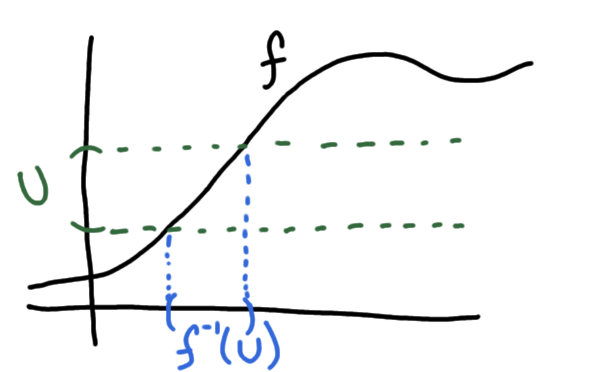
\includegraphics[width=4in]{toplec1_4.png}
\end{center}

Let's think a little about why it's open.  In the theorem, we do not assume that $U$ is an interval like in the picture.  To prove that $f^{-1}(U)$ is open, we need to show that for any $x$ in $f^{-1}(U)$ there is a little open interval around $x$ that is contained in $f^{-1}(U)$.

\begin{center}
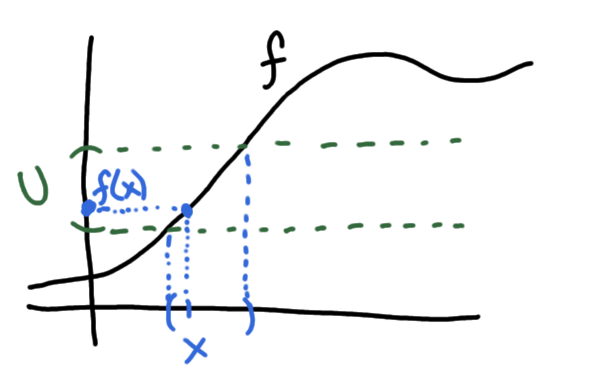
\includegraphics[width=4in]{toplec1_5.png}
\end{center}


An interval like that will look like this.  In the next image we see a little interval in red.  Any time a value $z$ is in that red interval, the function values $f(z)$ are inside $U$.  

\begin{center}
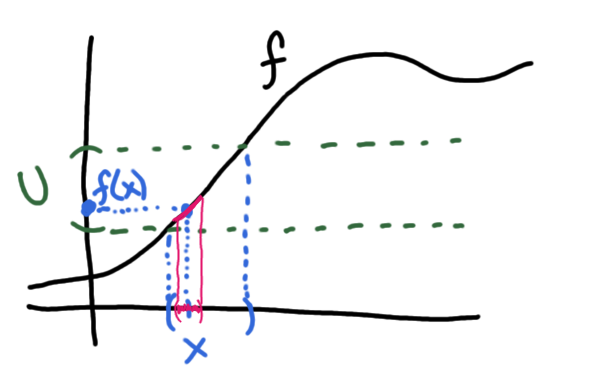
\includegraphics[width=4in]{toplec1_6.png}
\end{center}

Let's take one more step toward a formal proof.  Recall that $f(x)$ is in $U$ and $U$ is open.  That means we can produce a little open interval around $f(x)$ that is inside $U$.  In the next picture, we see a little $\epsilon$ interval $(f(x)-\epsilon, f(x)+\epsilon)$.  These are ``y''-values, so they are along the y axis.  

\begin{center}
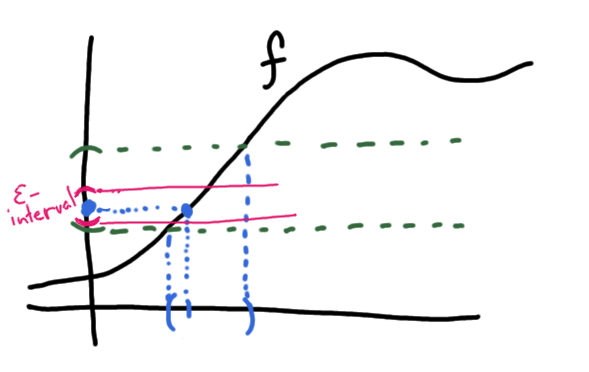
\includegraphics[width=4in]{toplec1_7.png}
\end{center}


Can we find a little $\delta$ interval around $x$ so that whenever $z$ is in  $(x-\delta,x+\delta)$ it follows that  $f(z)$ is in $(f(x)-\epsilon, f(x)+\epsilon)$?  If you are unsure, recall that this is exactly the definition of ``continuous at $x$''. 


\begin{center}
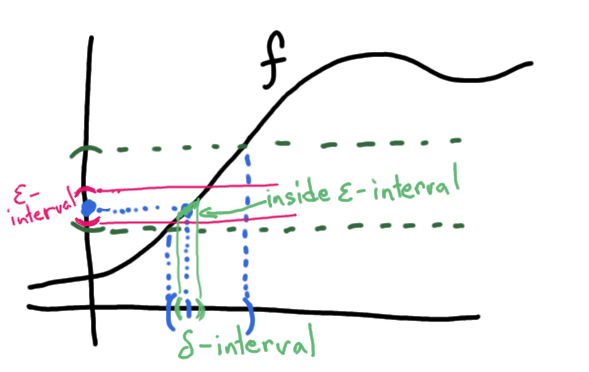
\includegraphics[width=4in]{toplec1_8.png}
\end{center}


If you understand this, then you will understand that the argument does not depend on our picture.  It works for any open set $U$.  


\subsection{The Role of Topology in Calculus}

Several of the most important ideas in calculus are basically topological---meaning to understand them the most natural thing is to use these ideas.  

Two of the most important examples: (1) the Intermediate Value Theorem, (2) the Extreme Value Theorem.


Here's why topology is useful in calculus.  So far we have defined everything \emph{pointwise}.  We defined continuity \emph{at x} and differentiability \emph{at x}, but some of the deeper theorems are about functions that are continuous \emph{everywhere}.  The Intermediate Value Theorem is not about any particular point, for example, and it's difficult to apply definitions of continuity that depend on some particular point $x$ when the theorem isn't about any particular point.  The alternative definition of continuous given in the theorem above allows us to take full advantage of functions that are continuous at every point in an interval.  

The ``topological'' method is an alternative point of view that will make the deeper theorems clearer if you can come to understand this point of view.  



\subsection{Exercises}

\begin{enumerate}
\item
Let $f(x)=\cos(x)$.  What is $f^{-1}(\{1\})$.  Here $\{1\}$ means the set containing just the number 1. Is $\{1\}$ open?  Is $f^{-1}(\{1\})$ open?




\item
Sketch an example of a function $f$ that is not continuous and some open set $U$ where $f^{-1}(U)$ is not open.  

\item
Refer to the theorem above about continuous functions.  If $U$ is not open, does that imply that $f^{-1}(U)$ is not open?

\item
Let $f(x)=x^2$.  Is $f$ continuous?  Let $U=(1,2)$. What is $f^{-1}(U)$?  Is $f^{-1}(U)$ open?  For this, don't just cite the theorem above, but convince yourself from the definition that it is open.



\end{enumerate}


\section{Extreme Value Theorem}


The Extreme Value Theorem is one of the foundational beams holding calculus up.  It's easy to state but very hard to prove (from the perspective of a calculus student).

\begin{theorem}
If $f$ is continuous on a closed interval $[a,b]$ then $f$ attains a global maximum and a global minimum.  
\end{theorem}

The word \emph{attains} in this theorem has a precise meaning.  We mean there is some $x$ in $[a,b]$ where $f(x)\leq f(a)$ for all $x\in [a,b]$.  We use \emph{attains} here to emphasize that $f$ actually equals its maximum at some point.  Contrast this with, for example, the function $arctan(x)$ which is bounded above by $\pi/2$ but never actually attains that value.  

In particular, this implies that $f$ is bounded.  

The Extreme Value Theorem is deep and topological in nature.  It's arguably the deepest theorem a calculus student would see, and therefore books tend to omit the proof.  

For the student who feels up to the challenge, we will try to push him in the right direction. 

The underlying idea behind the theorem is that a continuous function maps compact sets to compact sets, and in the real numbers, the compact sets are exactly the closed, bounded sets.  Thus, since $[a,b]$ is closed and bounded, $f([a,b])$ is also a closed, bounded set.

To prove the statement, however, we would make essential use of what \emph{compact} means.  We present the definition to give the reader an idea of the depth of the waters here.

\begin{definition}
A set $C$ is \emph{compact} if given any family $\{U_i\}$ of open sets that covers $C$, there is a finite subcollection $\{U_1, \ldots, U_p\}$ that covers $C$.  
\end{definition}

Here, ``cover'' means that $C$ is in the union.  


An alternative proof of the Extreme Value Theorem might rely on the statement that any sequence $\{x_i\}$ of points in $[a,b]$ has a convergent subsequence.  




\section{Topology for Calculus: Compactness}

In this section, we want to introduce the notion of \emph{compactness}.  It's fairly deep compared to the usual fare in calculus, but it's an essential idea to understand a proof of the extreme value theorem.

Calculus textbooks this author has seen do not bother to prove the extreme value theorem because it's surprisingly deep.  It's easy to state the theorem, and students usually readily believe it, but the proof does not really lie within the scope of calculus.

Most of the proofs we do in a calculus class are just simple manipulations of the $\epsilon$-$\delta$ sort.  To prove the extreme value theorem calls for tools of a more sophisticated nature.  The most natural approach is to use \hilight{compactness}.  So, if you want to understand the ideas at a deeper level, we offer you this visual introduction to the notion of compactness.  

\begin{definition}
An \emph{open cover} of a set $X$ is a family ${O_i}$ of open sets so that $X \subset \bigcup O_i$.
\end{definition}



In the following image is the set $X$, a closed rectangle.

\begin{center}
\begin{tikzpicture}
\filldraw[blue!40!white, draw=black] (0,0) rectangle (5,5);
\end{tikzpicture}
\end{center}

We cover it with open circles.  A mathematician would usually say ``open balls''.  We like to say ``circle'' or ``sphere'' for the boundary and ``ball'' for the points contained inside it.
``Cover'' means just what you think: every point of $X$ is contained in one of the open balls.

Here is a visual example of an open cover of $X$.  Obviously, it's easy to cover $X$ with just a finite number of open balls.  They don't have to be disjoint or anything.  They can overlap.  That's fine.


\begin{center}
\begin{tikzpicture}

\filldraw[blue!40!white, draw=black] (0,0) rectangle (5,5);



\fill[green,fill opacity=0.7] (1,4) circle(.5cm);
\fill[green,fill opacity=0.7] (2,4.5) circle(.3cm);
\fill[green,fill opacity=0.7] (2.5,4.5) circle(.15cm);
\fill[green,fill opacity=0.7] (2.7,4.5) circle(.075cm);
\fill[green,fill opacity=0.7] (4.5,.2) circle(1cm);
\fill[green,fill opacity=0.7] (.5,.5) circle(2cm);
\fill[green,fill opacity=0.7] (2,2) circle(1cm);

\fill[green,fill opacity=0.7] (1,4) circle(2cm);
\fill[green,fill opacity=0.7] (2,4) circle(.8cm);
\fill[green,fill opacity=0.7] (3.75,3.75) circle(2cm);


\fill[green,fill opacity=0.7] (3,0) circle(1.2cm);


\fill[green,fill opacity=0.7] (4,1) circle(2cm);

\end{tikzpicture}
\end{center}




Now, the following theorem is deep water---it's much deeper than what you would normally see in a calculus textbook.  So unless you want to study math further, we won't expect you to learn \emph{why} it's true:

\begin{theorem}
For any open cover $\{O_i\}$ of the closed rectangle $X$ in the picture, there is a finite subset $O_1,\ldots, O_n$ that covers $X$.
\end{theorem}


Let's try to understand that statement first because it's not the most intuitive idea in math.  \hilight{We are not saying that $X$ can be covered by a finite number of open balls.}  That's actually pretty obvious and so it isn't interesting.  

Think about the fact that you could imagine ways to use infinitely many balls to cover the rectangle.  They could get smaller and smaller.  There's no limit to how small they can be.  You can fill the rectangle with infinitely many super-tiny open balls. 

Obviously, a computer can't print infinitely many circles, but we hope the image below gives you the idea.




\begin{center}
\begin{tikzpicture}

\filldraw[blue!40!white, draw=black] (0,0) rectangle (5,5);



\fill[green,fill opacity=0.7] (1,4) circle(.5cm);
\fill[green,fill opacity=0.7] (2,4.5) circle(.3cm);
\fill[green,fill opacity=0.7] (2.5,4.5) circle(.15cm);
\fill[green,fill opacity=0.7] (2.7,4.5) circle(.075cm);
\fill[green,fill opacity=0.7] (4.5,.2) circle(1cm);
\fill[green,fill opacity=0.7] (.5,.5) circle(2cm);
\fill[green,fill opacity=0.7] (2,2) circle(1cm);
\fill[green,fill opacity=0.7] (3,3) circle(.5cm);
\fill[green,fill opacity=0.7] (3.5,3.5) circle(.25cm);
\fill[green,fill opacity=0.7] (3.75,3.75) circle(.12cm);
\fill[green,fill opacity=0.7] (3.9,3.9) circle(.06cm);

\end{tikzpicture}
\end{center}

The image above doesn't show an open cover.  You'd have to keep filling the page with more open balls to cover the rectangle.

In theory, you could cook up some infinite set of open balls $\{O_i\}$ and you could try to make it so that you need \emph{all} of them to cover the rectangle.  You might think if you are very clever and if the open balls just keep getting smaller and smaller, then you will need all of them to cover $X$.

But in fact you will not.  In fact, there will always be some finite number of them that cover the rectangle.  That's because the closed rectangle in the plane is \emph{compact}.

\begin{definition}
A set $X$  is \emph{compact} if for any open cover $\{O_i\}$ of $X$ there is a finite subset $\{O_1,\ldots, O_n\}$ that also covers $X$.  
\end{definition}

\hilight{And no amount of cleverness can make it so you \emph{have} to use all infinitely many of them.}  That is what compactness means.

\begin{theorem}
On the real line $\mathbb{R}$, every closed, bounded interval $[a,b]$ is compact.
\end{theorem}

\begin{theorem}
In the plane, $\mathbb{R}^2$ every closed, bounded set (such as the rectangle in the images) is compact.
\end{theorem}

The proofs of these theorems are not trivial, and they are rightfully beyond the scope of a calculus class.  If you want to learn more, you should consider studying math further.  You will learn about all these topics and more in a first course in topology.  If you want to learn on your own, a much-loved textbook is Munkre's \textit{Topology}.  

\subsection{Exercises}

\begin{enumerate}

\item
It's a doomed exercise, but go ahead and try to come up with an open cover of the interval $[0,1]$ where you actually need infinitely many sets to cover the closed interval.

You might attemt to make each interval half as long as the last one and try to arrange them all so that together they cover $[0,1]$.  We think it will be good for you to try this and see what difficulties arise.  




\end{enumerate}








\section{Exercises}

\begin{enumerate}

\item
Refer to the graphs.

\begin{center}
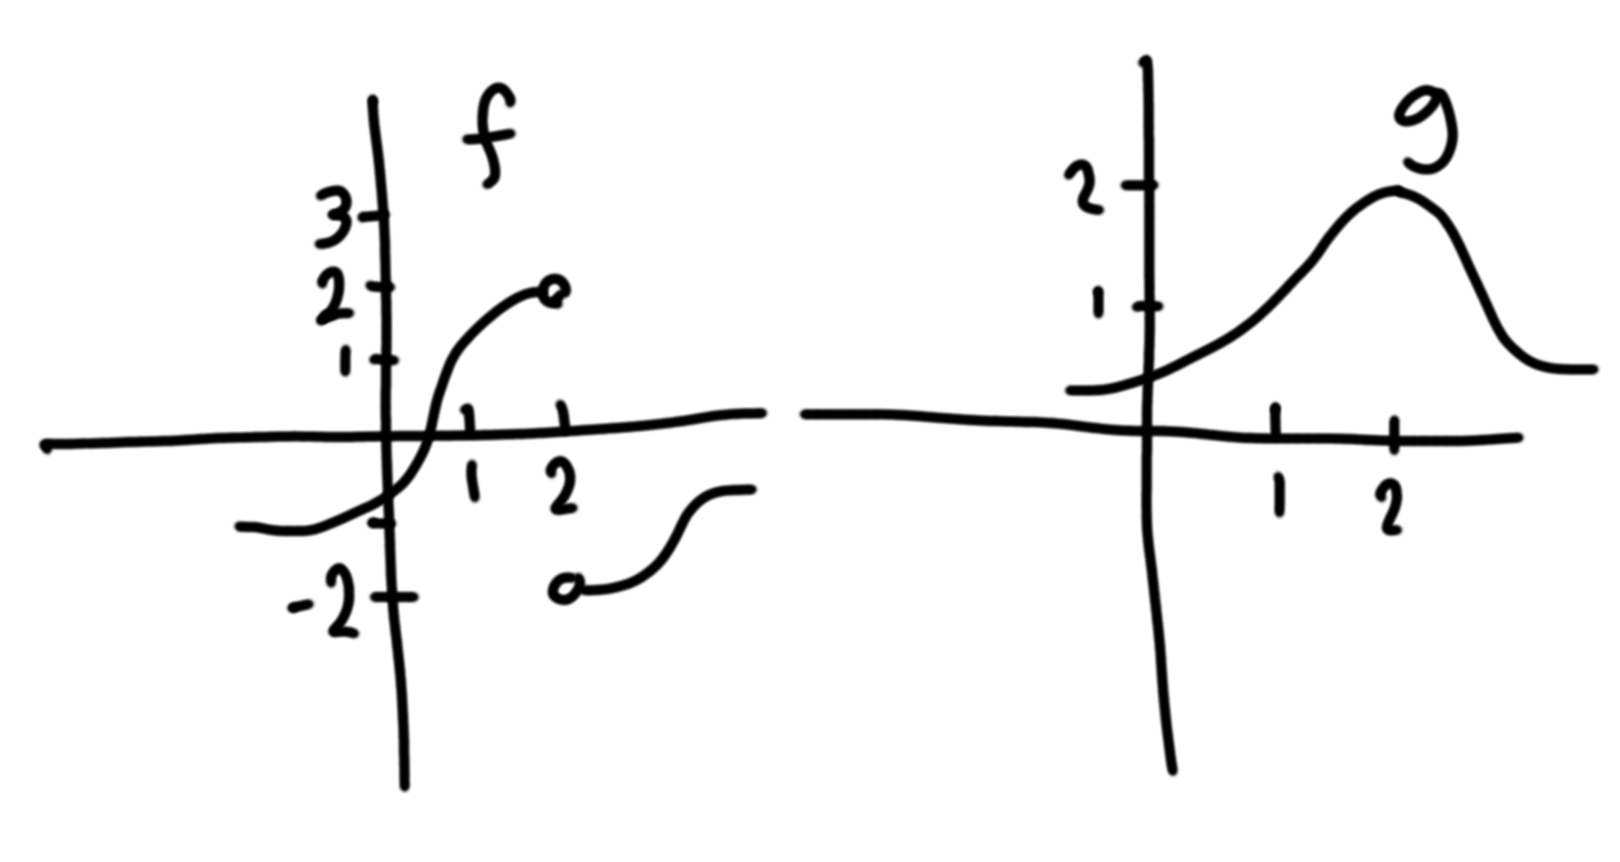
\includegraphics[width=4in]{limitExerciseImage1.png}
\end{center}

What is $\lim_{x\to 2} f(g(x))$?  What is $\lim_{x\to 2} g(f(x))$?




\item 

We will consider the limit $$\lim_{x\to 0} x^3.$$ 

\begin{enumerate}
\item 
Sketch a graph of $x^3$ around x=0 and draw two horizontal lines representing $\epsilon$ and $-\epsilon$. 



\item \label{b}
 What is the largest (most positive) value x can be so that   $x^3\leq \epsilon$?  
 

 
 \item \label{c}
  What is the most negative value x can be so that $x^3\geq -\epsilon$?



\item
What $\delta$ should we choose so that when $|x-0|<\delta$ we can be sure that $|x^3-0|<\epsilon$?  (Here we write the ``- 0'' part for emphasis so that it looks like the definition of a limit, but it can (and should) be omitted in most writing.  We want $\delta$ small so that $(x-\delta,x+\delta)$ is in the interval you identified in parts \ref{b} and \ref{c} above.



\item
If we require $|x^3-0|<1/1000$, how small does $|x|$ have to be?  



\end{enumerate}

\item

Explain in simple terms why $$\lim_{x\to 0} \frac{1}{x}$$ does not exist.  



\item
Explain in words why $$\lim_{x\to 0} x^2 \sin(2\pi/x)=0$$ (meaning the limit exists and is 0) but the limit $$\lim_{x\to 0} \sin(2\pi/x)$$ does not exist.  You are not required to write a proof, but explain what the essential difference is.









\end{enumerate}




\chapter{Derivatives}  

\section{Slope of the Tangent Line}

Given some function $f$, any two points on the curve determine a \emph{secant} line.  In the image below, $f(x)=\sin(x)$ and the two points pictured are $(\pi/2,1)$ and $(\pi/2+.5,\sin(\pi/2+.5))$.  


\begin{center}
\begin{tikzpicture}
  \draw[<->] (0,0) -- (6,0) node[right] {$x$};
  \draw[<->] (0,-1) -- (0,2) node[above] {$y$};

\draw (pi,-.2) -- (pi,.2); 
\node at (pi,-.5) {$\pi/2$};

%\draw (-1*2,1.629*2) -- (3*2,2*0.65);

\node[color=blue] at (2*pi/2,2*1) {\textbullet};
\node[color=red] at (2*2.07,2*.877) {\textbullet};
\draw[scale=2,domain=0:3,smooth,variable=\x,blue] plot ({\x},{sin(\x r)});

\draw[scale=2,domain=0:3,smooth,variable=\x,blue] plot ({\x},{1.38703-0.246392*\x});

\end{tikzpicture}
\end{center}

Recall how to conpute the slope of this line:

$$\frac{f(\pi/2+.5) - f(\pi/2)}{\pi/2+.5 - \pi/2}.$$
In this example, we think of $(\pi/2,1)$ as a fixed point we are interested in, and we pick another point close to it.  The $x$-coordinate differed by only a small number, 0.5.  It's traditional to use the letter $h$ to refer to that small number.  

If we choose an even smaller $h$, we get a different secant line.  Consider $h=0.3$.  In the next image, we have zoomed in close to $\pi/2$ and drawn the two secant lines given by $h=0.5$ and $h=0.3$.  


\begin{center}
\begin{tikzpicture}
\draw[<->] (-6,8) -- (6,8) node[right] {$x$};


%  \draw[<->] (0,-1) -- (0,2) node[above] {$y$};

%\draw (pi,-.2) -- (pi,.2); 
%\node at (pi,-.5) {$\pi/2$};

%\draw (-1*2,1.629*2) -- (3*2,2*0.65);

\node[color=blue] at (0,10) {\textbullet};


\node[color=red] at (10*.5,10*.877) {\textbullet};

\node[color=red] at (10*.3,10*.9553) {\textbullet};

\draw[scale=10,domain=-.5:.5,smooth,variable=\x,blue] plot ({\x},{sin((\x+pi/2) r)});

\draw[scale=10,domain=-.5:.5,smooth,variable=\x,blue] plot ({\x},{1.38703-0.246392*(\x+pi/2)});

\draw[scale=10,domain=-.5:.5,smooth,variable=\x,blue] plot ({\x},{1.23386-0.148878*(\x+pi/2)});


\end{tikzpicture}
\end{center}

Naturally, one might ask what happens as $h$ gets smaller and smaller.  Imagine the point at $(x+h,f(x+h))$ getting closer and closer to $(x,f(x)$.  What happens to the secant lines in the limit?  And what happens to the slope?  

In the example pictured, in the limit the secant lines go to a horizontal line.  We call this the tangent line.
\begin{center}
\begin{tikzpicture}
\draw[<->] (-6,8) -- (6,8) node[right] {$x$};


%  \draw[<->] (0,-1) -- (0,2) node[above] {$y$};

%\draw (pi,-.2) -- (pi,.2); 
%\node at (pi,-.5) {$\pi/2$};

%\draw (-1*2,1.629*2) -- (3*2,2*0.65);

\node[color=blue] at (0,10) {\textbullet};


\node[color=red] at (10*.5,10*.877) {\textbullet};

\node[color=red] at (10*.3,10*.9553) {\textbullet};

\draw[scale=10,domain=-.5:.5,smooth,variable=\x,blue] plot ({\x},{sin((\x+pi/2) r)});

\draw[scale=10,domain=-.5:.5,smooth,variable=\x,blue] plot ({\x},{1.38703-0.246392*(\x+pi/2)});

\draw[scale=10,domain=-.5:.5,smooth,variable=\x,blue] plot ({\x},{1.23386-0.148878*(\x+pi/2)});

\draw[scale=10,domain=-.5:.5,smooth,variable=\x,red] plot ({\x},{1});
\end{tikzpicture}
\end{center}


\begin{definition}
The \emph{tangent line of $f$ at $x$} is the limit of the secant line through $(x,f(x))$ and $(x+h,f(x+h))$ as $h$ goes to 0.  
\end{definition}

If the limit does not exist, then the tangent line is undefined.

In general the slope of the tangent line is the limit of the slope of the secant line:
$$\lim_{h\to 0} \frac{f(x+h)-f(x)}{h}$$




\begin{definition}
The \highlight{\emph{derivative of $f$ at $a$}} is 
$$f'(a)=\lim_{h\to 0} \frac{f(a+h)-f(a)}{h}$$
if the limit exists and is finite.
\end{definition}

If the limit doesn't exist or if it is infinite, we say the function is not \emph{differentiable} at $a$.

Students should memorize this definition.  It's very basic to an understanding of calculus.

We often use the notation $f'(x)$ for the derivative of $f$ at x.  We also use the notation $\frac{d}{dx}f(x)$ for the derivative of $f$ at $x$.  The two notations are used interchangeably.  Usually, when we use the $\frac{d}{dx}$ it's because we want to be explicit that we are taking the derivative \emph{with respect to $x$}.  We will talk about that more later.

In this section, we have learned one interpretation of the derivative of $f$ at $a$.  It is the slope of the tangent line at $a$.  We will learn some other interpretations in later sections.   

This expression 
$$\frac{f(x+h)-f(x)}{h}$$
is often called a \emph{difference quotient}.  As we have seen here, it's nothing but the familiar slope formula.  


\begin{example}
What is the derivative of $f(x)=x^{1/3}$ at 0?
\end{example}

\begin{center}
\begin{tikzpicture}
  \draw[<->] (-3,0) -- (3,0);
  \draw[<->] (0,-2) -- (0,2);
  
  \draw[<->,ultra thick, red] (0,-1) -- (0,1);

\node[color=blue] at (0,0) {\textbullet};

\draw[scale=2,domain=-1:1,samples=100,smooth,variable=\x,blue] plot ({\x},{\x^(1/3)});



\end{tikzpicture}
\end{center}


\begin{align*}
&\lim_{h\to 0}\frac{f(a+h)-f(a)}{h}\\
=&\lim_{h\to 0}\frac{h^{1/3}}{h}\\
=& \lim_{h\to 0} h^{-2/3}=\infty
\end{align*}

Since the limit is infinite, the derivative does not exist.  This corresponds to the vertical tangent line at 0.

\begin{example}
Let $f(x)=x^2$ with the domain $[-1,1]$.  What is $f'(1)$?

\end{example}



\section{Ways a Function Might Not be Differentiable}


In the previous section, we saw the function $f(x)=x^{1/3}$, which is not differentiable at 0 because the tangent line has infinite slope at that point.  

In this section, we will consder other ways a function may fail to be differentiable.  In all cases, however, this reduces to showing that
$$\lim_{h\to 0}\frac{f(a+h)-f(a)}{h}$$
is infinite or does not exist.

\subsection{A Sharp Point}

The function $f(x)=|x|$ is not differentiable at 0.  The intuitive reason is that $f$ has a point there.  You might say there is no way to define a tangent line at 0.  

That kind of reasoning may be acceptable in a high school calculus class, but at the college level, you should be able to show from the definition that the derivative does not exist.

\begin{example}
Show that function $f(x)=|x|$ is not differentiable at 0.
\end{example}

How do we start?  (Try to answer before you continue reading.)

We write down the definition of the derivative at 0:
$$f'(0) = \lim_{h\to 0}\frac{|0+h|-|0|}{h}= \lim_{h\to 0}\frac{|h|}{h}$$

One way a limit may fail to exist is if the left hand limit and the right hand limit are not the same.  Recall that when $h>0$ we can write $|h|=h$ and when $h<0$ we can write $|h|=-h$.  Thus
$$\lim_{h\to 0^+}\frac{|h|}{h}=\lim_{h\to 0+}\frac{h}{h}=1$$ 
and 
$$\lim_{h\to 0^-}\frac{|h|}{h}=\lim_{h\to 0+}\frac{-h}{h}=-1.$$ 



Since the left and right limits are not equal, the limit does not exist, so the derivative does not exist at 0.  


\begin{error}
When presented with this argument, students often get confused about whether $\lim_{x\to 0} |x|$ exists.  In fact, it does.  The function $f(x)=|x|$ is continuous everywhere.  When talking about the derivative at 0, we take the limit of $\frac{f(h)-f(0)}{h}$.  It's \emph{this} limit that doesn't exist.  

\end{error}



This argument is completely sufficient, but let's also think about secant lines.  If $h$ is any positive number, then the secant line through the points $(0,0)$ and $(h,|h|)$ is always $y=x$.  That's true no matter how small $h$ is, so long as it is positive. 


\begin{center}
\begin{tikzpicture}
  \draw[<->] (-2,0) -- (2,0);
  \draw[<->] (0,-1) -- (0,2) ;


\draw[<->, ultra thick, red] (-1,-1) -- (1,1) ;

\node[color=blue] at (0,0) {\textbullet};

\node[color=red] at (.5,.5) {\textbullet};

\draw[scale=1,domain=-2:2,smooth,variable=\x,blue] plot ({\x},{abs(\x)});




\end{tikzpicture}
\end{center}


Now think about a negative $h$.  In this case, the secant line has slope -1 no matter how small $h$ is.



\begin{center}
\begin{tikzpicture}
  \draw[<->] (-2,0) -- (2,0);
  \draw[<->] (0,-1) -- (0,2) ;


\draw[<->, ultra thick, red] (-1,1) -- (1,-1) ;

\node[color=blue] at (0,0) {\textbullet};

\node[color=red] at (-.5,.5) {\textbullet};

\draw[scale=1,domain=-2:2,smooth,variable=\x,blue] plot ({\x},{abs(\x)});
\end{tikzpicture}
\end{center}
So the secant lines don't approach any single tangent line.  

\subsection{Oscillating Secant}


Consider $f(x)=x\sin(1/x)$.  This function oscillates infinitely many times between the two lines $y=x$ and $y=-x$ so that around $x=0$ you can't even really graph it, but we can give the idea of it in the following image.



\begin{center}
\begin{tikzpicture}


%\draw[scale=100,domain=0.001:0.1,smooth,samples=50,variable=\x,blue] plot ({\x},{1/100*sin((1/\x) r)});

\begin{axis}[samples=1000,
axis x line=center,
y=12.5in,
x=25in,
axis y line=center,
xmin=0,
xmax=0.1,
ymin=-.1,
ymax=.1,restrict y to domain =-2:2]
\addplot[very thick,blue,domain=0.0004:.1]plot (\x, {\x*sin((1/\x r))});

\addplot[ultra thick,blue,domain=0:0.070735]plot (\x, {\x});

\addplot[ultra thick,blue,domain=0:0.090945681766]plot (\x, {-\x});


\end{axis}
\draw[red,fill=red] (0.070735*25in,1.25in +12.5*0.070735 in) circle (.05in);

\draw[red,fill=red] (0,1.25in) circle (.05in);

\draw[red,fill=red] (0.090945681766*25in,.113 in) circle (.05in);



\end{tikzpicture}
\end{center}

No matter how much you zoom it, it still looks basically the same: the oscillations bunch up tighter and tighter at 0.  Also, no matter how close we zoom in, there are some values of $x$ where $\sin(1/x)=1$ and others where $\sin(1/x)=-1$.  Those are places where $x\sin(1/x)$ touches the bounding lines $y=x$ and $y=-x$.

In the figure, we illustrated two secant lines.  At $x_n=\frac{1}{\pi(4n+1)}$ we have $f(x_n)=x_n$.  In the figure, we have drawn $(x_2,f(x_2)$ and you can see that the secant line between $(0,0)$ and $(x_2,f(x_2)$ has slope 1.  

However, at $z_n=\frac{2}{\pi(4n-1)}$ we have $f(z_n)=-z_n$.  We have drawn the point $(z_2,f(z_2)$  The secant line between $(0,0)$ and $(z_2,f(z_2)$ has slope -1.  

The derivative of $f$ at 0 does not exist in this example because no matter how close $h$ is to 0, there are always some values of $h$ where 
$$\frac{f(h)-f(0)}{h}=1$$
and some values of $h$ where 
$$\frac{f(h)-f(0)}{h}=-1.$$
Since they are not zeroing in toward a single number, the limit does not exist.  

Contrast with the function $f(x)=x^2\sin(1/x)$ which \emph{is} differentiable at 0.  

\section{The Product Rule}

\begin{prop}
If $f$ and $g$ are differentiable at $x$ then 
$$\frac{d}{dx}[f(x)g(x)]=f'(x)g(x)+f(x)g'(x).$$

\end{prop}

\begin{error}
Students often want the derivative of $f(x)g(x)$ to be $f'(x)g'(x)$.  That would be easy, but it just isn't true.    
\end{error}


\begin{center}
\begin{tikzpicture}
\filldraw[blue!40!white, draw=black] (0,0) rectangle (4,4);
\filldraw[blue!40!red, draw=black] (4,0) rectangle (5,4);

\filldraw[blue!40!green, draw=black] (0,4) rectangle (4,5);

\filldraw[cyan!40!green, draw=black] (0,4) rectangle (4,5);

\filldraw[blue!40!green, draw=black] (4,4) rectangle (5,5);

\draw [decorate,decoration={brace,amplitude=10pt}] (-.2,0) -- (-.2,4);

\draw [decorate,decoration={brace,amplitude=10pt}] (-1.3,0) -- (-1.3,5);

\draw [decorate,decoration={brace,amplitude=10pt,mirror}] (0,-.3) -- (4,-.3);

\draw [decorate,decoration={brace,amplitude=10pt,mirror}] (0,-1.3) -- (5,-1.3);


\node at (-2.5,2.5) {$f(a+h)$};

\node at (-1,2) {$f(a)$};
\node at (2,-1) {$g(a)$};
\node at (2,2) {$A$};
\node at (-.4,4.5) {$\Delta f$};
\node at (4.5,2) {$B$};

\node at (2.5,-2) {$g(a+h)$};
\node at (2,4.5) {$C$};
\node at (4.5,4.5) {$D$};
\node at (4.5,-.3) {$\Delta g$};
\end{tikzpicture}
\end{center}


We present a visual argument that isn't completely general.  My students have found it illuminating. 

By definition, the derivative of $f(x)g(x)$ at $a$ is
$$\lim_{h\to 0}\frac{f(a+h)g(a+h)-f(a)g(a)}{h}.$$
Let's assume for the moment that the numbers are all positive so we can illustrate them with rectangles as in the figure.

Observe that $f(a+h)g(a+h)$ is the combined area of the four rectangles A, B, C and D while $f(a)g(a)$ is the area of just rectangle A.  Therefore, $f(a+h)g(a+h)-f(a)g(a)$ is the area of B + C + D.  

Now, it's easy to see that $C=g(a)(f(a+h)-f(a))$ and $B=f(a)(g(a+h)-g(a))$ and $D=(f(a+h)-f(a))(g(a+h)-g(a))$.  To compute the limit above, we take 
$$\lim_{h\to 0} \frac{B+C+D}{h}.$$

Now, we see that 
$$\lim_{h\to 0} \frac{B}{h}=\lim_{h\to 0} \frac{f(a)(g(a+h)-g(a))}{h}=f(a)g'(a).$$
Similarly
$$\lim_{h\to 0} \frac{C}{h}=\lim_{h\to 0} \frac{g(a)(g(a+h)-g(a))}{h}=g(a)f'(a).$$
Finally
$$\lim_{h\to 0} \frac{D}{h}=\lim_{h\to 0} \frac{g(a+h)-g(a)}{h}(f(a+h)-f(a))=0.$$

Therefore the derivative at $a$ is $f(a)g'(a)+g(a)f'(a)$.

Note that to draw the visual in terms of areas of rectangles, we made assumptions about things being positive, but that really played no role in the argument.  $f(a+h)g(a+h)-f(a)g(a) = $

\section{The Chain Rule}


\begin{prop}
If $f$ and $g$ are differentiable then $\frac{d}{dx}f(g(x)) = f'(g(x))g'(x)$.
\end{prop}

\begin{example}

Compute the derivative $\frac{d}{dx}\sin(x^2)$.

The outside function in this composition is $f(x)=\sin(x)$.  The inside function is $g(x)=x^2$.  Thus $\frac{d}{dx}\sin(x^2) = f'(g(x))g'(x)= \cos(x^2)(2x)$.

\end{example}

\begin{error}
Students often get confused in applying the chain rule.  You have to keep in mind that what goes inside $f'$ is $g(x)$, not $g'(x)$.  A common error is to say the derivative is $f'(g'(x))$, but you should be careful.  That's not what the chain rule says.
\end{error}





The following proof sketch is intended to be illuminating rather than exactly precise.  An exactly precise proof would be written with $\epsilon$s and $\delta$s, but we think the student is more likely to undestand the idea presented this way.

\begin{proof}[Proof Sketch]

Since $g'(x)$ exists, for $h$ small, 
$$\frac{g(x+h)-g(x)}{h}\approx g'(x).$$

Here the $\approx$ symbol means ``is approximately''.  Therefore, 
$$g(x+h)-g(x)\approx hg'(x)$$
and 
$$g(x+h)\approx hg'(x)+g(x).$$

To compute the derivative of $f(g(x))$ at $x$, the difference quotient is $$\frac{f(g(x+h))-f(g(x))}{h}.$$
For $h$ small, 
$$ 
\frac{f(\highlight{g(x+h)})-f(g(x))}{h} \approx \frac{f(\highlight{g(x) + hg'(x)})-f(g(x))}{h}.$$
Observe we have just replaced $g(x+h)$ with $g(x) + hg'(x)$.  Next we multiply top and bottom by $g'(x)$ and we have 
\begin{equation} \label{3240972392408}
\frac{f(g(x) + hg'(x))-f(g(x))}{hg'(x)} g'(x).
\end{equation}

The quotient on the left in  (\ref{3240972392408}) almost has the form of a difference quotient.  As $h\to 0$, we also see that $hg'(x)\to 0$ so 
$$\lim_{h\to 0} \frac{f(g(x) + hg'(x))-f(g(x))}{hg'(x)}  = \lim_{h\to 0} \frac{f(g(x) + h)-f(g(x))}{h} = f'(g(x)).$$
Those limits are the same because it doesn't really matter what symbol appears in the highlighted portion of the difference quotient: 
$$\frac{f(g(x) + \highlight{hg\prime(x)})-f(g(x))}{\highlight{hg'(x)}}.$$
It only matters that those two numbers are the \emph{same} and that they are going to zero in the limit.  That's why we had to multiply and divide by $g'(x)$.  We needed to have the same number in those two highlighted positions.  

Thus $\frac{d}{dx}f(g(x)) = f'(g(x))g'(x)$.
\end{proof}

\section{Practice Quiz}

For the best learning experience, treat a practice quiz like an in-class quiz. Don't refer to other parts of the textbook.

\begin{enumerate}


\item Circle T for true or F for false:
\begin{enumerate}
\item T/F For any numbers $a$ and $b$, where $a<b$, there is a rational number $p/q$ so that $a<p/q<b$.

\item T/F The number $\sqrt{2}$ can be written as $p/q$ where $p$ and $q$ are both integers.

\item T/F The limit $\lim_{n\to \infty} (1+1/n)^{n}$ does not exist.

\item T/F It's possible to find a rational number as close to $\pi$ as you want.

\end{enumerate}


\item Compute the derivative.  

\begin{enumerate}
\item
$\frac{d}{dx} e^{\sin(x)}$
\item
$\frac{d}{dx} \ln(\cos(x))$
\item
$\frac{d}{dx} x^3\tan(x)$
\item
$\frac{d}{dx} \sin(x)^x$
\end{enumerate}




\item
Compute the derivative $\frac{d}{dx} \sin^{-1}(x)$ using the chain rule/implicit differentiation technique.  



\item Let's think about how to approximate $\sin(1^\circ)$.

\begin{enumerate}


\item  Since $1^\circ$ is close to $0^\circ$, we will find a tangent line at 0.  But why is $0^\circ$ any easier than $1^\circ$?



\item What is the slope of the tangent line at $0$?



\item What is the equation of the tangent line at $0$?



\item What is the value of the tangent line at $1^\circ$?  (Be sure to convert into radians.)



\item Why is your answer in the previous part a reasonable approximation to $\sin(1^\circ)$?

\end{enumerate}


\end{enumerate}



\section{Extreme Values}


We say a function $f$ has a \emph{local maximum} at a point $a$ if there is an interval $(a-\epsilon,a+\epsilon)$ around $a$ where $f(x)\leq f(a)$ for all $x$ in $(a-\epsilon,a+\epsilon)$ and in the domain of $f$. 

Another way to say this is $f(x)\leq f(a)$ in a neighborhood of $a$.  

A \emph{local maximum} is defined similarly.  


We say $f$ has a \emph{global maximum} at $a$ if $f(x)\leq f(x)$ for all $x$ in the domain of $f$.  

A \emph{global maximum} is defined similarly.  

\begin{example}

In the following example, $f$ is defined on $[-2.5,2]$.  There are local maxima at $a$ and $2$.  There are local minima at $b$ and $-2.5$.  The global max is at $a$.  The global min is at $-2.5$.  




\begin{center}
\begin{tikzpicture}
  \draw[<->] (-4,0) -- (3,0) node[right] {$x$};
  \draw[<->] (0,-1) -- (0,2) node[above] {$y$};

\draw (-.8685,-0.1) -- (-.8685,0.1)
node[below=0.1in] {$a$};

\draw (1.54,-0.1) -- (1.54,0.1)
node[below=0.1in] {$b$};

\draw (-2.5,-0.1) -- (-2.5,0.1)
node[below=0.1in] {$-2.5$};

\draw (2,-0.1) -- (2,0.1)
node[below=0.1in] {$2$};

\draw[scale=1,domain=-2.5:2,smooth,variable=\x,blue] plot ({\x},{1/5*(\x+2)*(\x-1)*(\x-2)});

\node[color=black] at (-2.5,2) {$f$};

\node[color=blue] at (-2.5,-1.57) {\textbullet};

\node[color=blue] at (2,0) {\textbullet};

\end{tikzpicture}
\end{center}

\end{example}


\begin{prop}
If $f$ is defined on an interval $[a,b]$ and $f$ has a local minimum or a local maximum at $c \in [a,b]$, where $c$ is not one of the endpoints, and if $f$ is differentiable at $c$ then $f'(c)=0$.   
\end{prop}

Why did we assume $c$ isn't an endpoint?  Consider $f(x)=x^2$ restricted to the domain $[-2,2]$.  Then $f$ has a local (and global) max at $x=2$, but the derivative at $2$ is $f'(2)=4$.  

\begin{center}
\begin{tikzpicture}
  \draw[<->] (-3,0) -- (3,0) node[right] {$x$};
  \draw[<->] (0,-1) -- (0,4.2) node[above] {$y$};
\draw (-2,-0.1) -- (-2,0.1)
node[below=0.1in] {-2};
\draw (2,-0.1) -- (2,0.1)
node[below=0.1in] {2};
\node[color=blue] at (-2,4) {\textbullet};
\node[color=blue] at (2,4) {\textbullet};
\draw[scale=1,domain=-2:2,smooth,variable=\x,blue] plot ({\x},{\x*\x});
\end{tikzpicture}
\end{center}

Is it possible that $f$ has a local maximum at $a$ but $f'(a)$ doesn't exist?  Consider $f(x)=|x|$, which has a local minimum at 0, but $f'(0)$ does not exist.  So we have to assume $f'(a)$ exists.  

\begin{center}
\begin{tikzpicture}
  \draw[<->] (-3,0) -- (3,0) node[right] {$x$};
  \draw[<->] (0,-1) -- (0,3) node[above] {$y$};
\draw (-2,-0.1) -- (-2,0.1)
node[below=0.1in] {-2};
\draw (2,-0.1) -- (2,0.1)
node[below=0.1in] {2};
\node[color=blue] at (-2,2) {\textbullet};
\node[color=blue] at (2,2) {\textbullet};
\draw[scale=1,domain=-2:2,smooth,variable=\x,blue] plot ({\x},{abs(\x)});
\end{tikzpicture}
\end{center}

\begin{proof}
Assume $f$ has a local maximum at $c$.  We consider the limit of $\frac{f(c+h)-f(c)}{h}$ as $h\to 0$ from the right and from the left.  

If $h>0$ and $h$ is small enough, then 
$$\frac{f(c+h)-f(c)}{h}\leq 0.$$
Consider the slope of the secant line in the following illustration.

\begin{center}
\begin{tikzpicture}
  \draw[<->] (-2,0) -- (3,0) node[right] {$x$};
  \draw[<->] (0,-1) -- (0,2) node[above] {$y$};

\draw (pi/2,-0.1) -- (pi/2,0.1)
node[below=0.1in] {$\pi/2$};

\draw (-1,1.629) -- (3,0.65);
\node[color=blue] at (pi/2,1) {\textbullet};
\node[color=red] at (2.07,.877) {\textbullet};
\draw[scale=1,domain=-2:3,smooth,variable=\x,blue] plot ({\x},{sin(\x r)});
\end{tikzpicture}
\end{center}

Thus $$\lim_{h\to 0^+}\frac{f(c+h)-f(c)}{h}\leq 0.$$

On the other hand, if $h<0$ then 
$$0\leq \frac{f(c+h)-f(c)}{h}.$$


\begin{center}
\begin{tikzpicture}
  \draw[<->] (-2,0) -- (3,0) node[right] {$x$};
  \draw[<->] (0,-1) -- (0,2) node[above] {$y$};

\draw (pi/2,-0.1) -- (pi/2,0.1)
node[below=0.1in] {$\pi/2$};

\draw (-1,.36) -- (3,1.35);
\node[color=blue] at (pi/2,1) {\textbullet};
\node[color=red] at (1.07,.877) {\textbullet};

\draw[scale=1,domain=-2:3,smooth,variable=\x,blue] plot ({\x},{sin(\x r)});
\end{tikzpicture}
\end{center}


Thus $$0\geq \lim_{h\to 0^-}\frac{f(c+h)-f(c)}{h}.$$
Since the limit exists, the right hand limit and the left hand limit are the same, so 
$$0\leq \lim_{h\to 0}\frac{f(c+h)-f(c)}{h} \leq 0$$
so $f'(c)=0$.

The argument is the same when $f$ has a local minimum at $c$.  The only difference is that the inequalities are flipped.  

\end{proof}

\section{Indeterminate forms and L'H\^{o}pital's Rule}

How can we evaluate limits like 
$$\lim_{x\to \infty} \frac{e^x}{x^2}?$$
The difficulty here is that both numerator and denominator are going to $infinity$, and $\infty/\infty$ tells us nothing.  In general, a limit of that form could $infinity$ or 0 or any finite number, and so far we haven't developed any tools for dealing with that.  


Enter L'H\^{o}pital's Rule.  It's a theorem that allows us to evaluate these limits by taking derivatives, and we use it \emph{all the time}.  

\subsection{Indeterminate Forms}

Let's back up and make sure we understand indeterminate forms.  For shorthand, we often write $\frac{\infty}{\infty}$, but keep in mind that what we really mean is we have some functions $f$ and $g$ and we're taking a limit $\lim_{x\to a}\frac{f(x)}{g(x)}$ where both $f$ and $g$ go to infinity.

Infinity isn't a number, so it doesn't actually make any sense to do division.  We can only make sense of $\frac{\infty}{\infty}$ in terms of limits in a particular situation.

Another indeterminate form is $\frac{0}{0}$.  This one means we have some limit  $\lim_{x\to a}\frac{f(x)}{g(x)}$ where $f$ and $g$ both go to 0.  An example is $$\lim_{x\to 0}\frac{\sin(x)}{x}.$$

A third indeterminate form is $0\cdot \infty$.  An example is 
$$\lim_{x\to 0}e^{1/x^2}\sin(x).$$


\begin{error}
The forms $\frac{\infty}{0}$ and $\frac{0}{\infty}$ are \emph{not} indeterminate.  For example, if $f\to 0$ and $g\to \infty$ then $\frac{f}{g}\to 0$ unambiguously.  The two functions don't compete.  Both $f$ going to 0 and $g$ going to $\infty$ tend to make the ratio small.
\end{error}

\subsection{L'H\^{o}pital's Rule}


\begin{theorem}
If $f$ and $g$ are both differentiable and if $\lim_{x\to a} \frac{f(x)}{g(x)}$ has one of the indeterminate forms $\frac{\infty}{\infty}$ or $\frac{0}{0}$ then 
$$\lim_{x\to a} \frac{f(x)}{g(x)} = \lim_{x\to a} \frac{f'(x)}{g'(x)}.$$
Here $a$ may be any number or $\pm\infty$.
\end{theorem}

\begin{error}
You \emph{have} to verify that $\lim_{x\to a} \frac{f(x)}{g(x)}$ has an indeterminate form $\frac{\infty}{\infty}$ or $\frac{0}{0}$ before you can apply L'H\^{o}pital's Rule.  If you don't, you may get false results.  
\end{error}


\subsection{Proof of L'H\^{o}pital's Rule}

We're actually not going to \emph{prove} L'H\^{o}pital's rule in full generality and completely precisely.  What we will do is think about the main ideas of the proof.  Your main goal as you read this is to \hilight{understand how the Mean Value Theorem shows up in this argument}.

We also choose to write in the style below, using the notion of ``$\approx$'', or ``approximately equals'' rather than the more precise $\epsilon$-$\delta$ approach, because (1) working mathematicians often think like this and (2) we think it may actually make more sense to a beginning students than the $\epsilon$-$\delta$ approach.

We begin a proof sketch of the $\frac{\infty}{\infty}$ case.

Assume both limits $\lim_{x\to \infty}f'(x)$ and $\lim_{x\to \infty}g'(x)$ exist.  For shorthand, let's call them $f'(\infty)$ and $g'(\infty)$.  Then there exists $M$ so that whenever $x>M$ it follows that $g'(x)$ is close to $g'(\infty)$ and $f'(x)$ is close to $g'(\infty)$.

Now consider any interval $[a,b_n]$ where $M<a$ and  $b_n=n$, any integer bigger than $n$.    


Note that 
$$\frac{f(b_n)-f(a)}{g(b_n)-b(a)} = 
\frac{\frac{f(b_n)-f(a)}{b_n-a}}{\frac{g(b_n)-g(a)}{b_n-a}}$$
and by the Mean Value Theorem there are points $x^*_n$ and $z^*_n$ in $(a,b_n)$ where $$\frac{f(b_n)-f(a)}{b_n-a}=f'(x^*_n)$$
and 
$$\frac{g(b_n)-g(a)}{b_n-a}=g'(z^*_n).$$
Then, since $M<x^*_n,z^*_n$, we know that 
$$\frac{f(b_n)-f(a)}{b_n-a}\approx f'(\infty)$$
and 
$$\frac{g(b_n)-g(a)}{b_n-a}\approx g'(\infty)$$
so 
\begin{equation}\label{4907208720394}\frac{f(b_n)-f(a)}{g(b_n)-b(a)} \approx \frac{f'(\infty)}{g'(\infty)}.\end{equation}

Now, the approximate equality (\ref{4907208720394}) holds no matter what $n$ is.  As $n\to \infty$ gets bigger, $f(b_n)\to \infty$ and $g(b_n)\to\infty$.  But $f(a)$ and $g(a)$ stay the same.

We claim that $$\lim_{n\to \infty}\frac{f(b_n)-f(a)}{g(b_n)-b(a)} = \lim_{n\to \infty}\frac{f(b_n)}{g(b_n)}.$$
The essential point of this idea is that as $f(b_n)$ gets bigger and bigger, subtracting $f(a)$ makes less and less difference.  Think about what happens to $\frac{x-5}{x+30}$ as $x\to \infty$.  In the long run, the -5 and the +30 are irrelevant, right?  The limit is just 1. 

Therefore, $$ \lim_{n\to \infty}\frac{f(b_n)}{g(b_n)} \approx \frac{f'(\infty)}{g'(\infty)}.$$  
Since we can make this approximation as close as we want by choosing $M$ big enough, 
$$ \lim_{n\to \infty}\frac{f(b_n)}{g(b_n)} = \frac{f'(\infty)}{g'(\infty)}.$$




\chapter{Integrals}


\chapter*{GNU Free Documentation License}
\phantomsection  % so hyperref creates bookmarks

%\label{label_fdl}

 \begin{center}

       Version 1.3, 3 November 2008


 Copyright \copyright{} 2000, 2001, 2002, 2007, 2008  Free Software Foundation, Inc.
 
 \bigskip
 
     \texttt{<http://fsf.org/>}
  
 \bigskip
 
 Everyone is permitted to copy and distribute verbatim copies
 of this license document, but changing it is not allowed.
\end{center}


\begin{center}
{\bf\large Preamble}
\end{center}

The purpose of this License is to make a manual, textbook, or other
functional and useful document ``free'' in the sense of freedom: to
assure everyone the effective freedom to copy and redistribute it,
with or without modifying it, either commercially or noncommercially.
Secondarily, this License preserves for the author and publisher a way
to get credit for their work, while not being considered responsible
for modifications made by others.

This License is a kind of ``copyleft'', which means that derivative
works of the document must themselves be free in the same sense.  It
complements the GNU General Public License, which is a copyleft
license designed for free software.

We have designed this License in order to use it for manuals for free
software, because free software needs free documentation: a free
program should come with manuals providing the same freedoms that the
software does.  But this License is not limited to software manuals;
it can be used for any textual work, regardless of subject matter or
whether it is published as a printed book.  We recommend this License
principally for works whose purpose is instruction or reference.


\begin{center}
{\Large\bf 1. APPLICABILITY AND DEFINITIONS\par}
\phantomsection
\end{center}

This License applies to any manual or other work, in any medium, that
contains a notice placed by the copyright holder saying it can be
distributed under the terms of this License.  Such a notice grants a
world-wide, royalty-free license, unlimited in duration, to use that
work under the conditions stated herein.  The ``\textbf{Document}'', below,
refers to any such manual or work.  Any member of the public is a
licensee, and is addressed as ``\textbf{you}''.  You accept the license if you
copy, modify or distribute the work in a way requiring permission
under copyright law.

A ``\textbf{Modified Version}'' of the Document means any work containing the
Document or a portion of it, either copied verbatim, or with
modifications and/or translated into another language.

A ``\textbf{Secondary Section}'' is a named appendix or a front-matter section of
the Document that deals exclusively with the relationship of the
publishers or authors of the Document to the Document's overall subject
(or to related matters) and contains nothing that could fall directly
within that overall subject.  (Thus, if the Document is in part a
textbook of mathematics, a Secondary Section may not explain any
mathematics.)  The relationship could be a matter of historical
connection with the subject or with related matters, or of legal,
commercial, philosophical, ethical or political position regarding
them.

The ``\textbf{Invariant Sections}'' are certain Secondary Sections whose titles
are designated, as being those of Invariant Sections, in the notice
that says that the Document is released under this License.  If a
section does not fit the above definition of Secondary then it is not
allowed to be designated as Invariant.  The Document may contain zero
Invariant Sections.  If the Document does not identify any Invariant
Sections then there are none.

The ``\textbf{Cover Texts}'' are certain short passages of text that are listed,
as Front-Cover Texts or Back-Cover Texts, in the notice that says that
the Document is released under this License.  A Front-Cover Text may
be at most 5 words, and a Back-Cover Text may be at most 25 words.

A ``\textbf{Transparent}'' copy of the Document means a machine-readable copy,
represented in a format whose specification is available to the
general public, that is suitable for revising the document
straightforwardly with generic text editors or (for images composed of
pixels) generic paint programs or (for drawings) some widely available
drawing editor, and that is suitable for input to text formatters or
for automatic translation to a variety of formats suitable for input
to text formatters.  A copy made in an otherwise Transparent file
format whose markup, or absence of markup, has been arranged to thwart
or discourage subsequent modification by readers is not Transparent.
An image format is not Transparent if used for any substantial amount
of text.  A copy that is not ``Transparent'' is called ``\textbf{Opaque}''.

Examples of suitable formats for Transparent copies include plain
ASCII without markup, Texinfo input format, LaTeX input format, SGML
or XML using a publicly available DTD, and standard-conforming simple
HTML, PostScript or PDF designed for human modification.  Examples of
transparent image formats include PNG, XCF and JPG.  Opaque formats
include proprietary formats that can be read and edited only by
proprietary word processors, SGML or XML for which the DTD and/or
processing tools are not generally available, and the
machine-generated HTML, PostScript or PDF produced by some word
processors for output purposes only.

The ``\textbf{Title Page}'' means, for a printed book, the title page itself,
plus such following pages as are needed to hold, legibly, the material
this License requires to appear in the title page.  For works in
formats which do not have any title page as such, ``Title Page'' means
the text near the most prominent appearance of the work's title,
preceding the beginning of the body of the text.

The ``\textbf{publisher}'' means any person or entity that distributes
copies of the Document to the public.

A section ``\textbf{Entitled XYZ}'' means a named subunit of the Document whose
title either is precisely XYZ or contains XYZ in parentheses following
text that translates XYZ in another language.  (Here XYZ stands for a
specific section name mentioned below, such as ``\textbf{Acknowledgements}'',
``\textbf{Dedications}'', ``\textbf{Endorsements}'', or ``\textbf{History}''.)  
To ``\textbf{Preserve the Title}''
of such a section when you modify the Document means that it remains a
section ``Entitled XYZ'' according to this definition.

The Document may include Warranty Disclaimers next to the notice which
states that this License applies to the Document.  These Warranty
Disclaimers are considered to be included by reference in this
License, but only as regards disclaiming warranties: any other
implication that these Warranty Disclaimers may have is void and has
no effect on the meaning of this License.


\begin{center}
{\Large\bf 2. VERBATIM COPYING\par}
\phantomsection

\end{center}

You may copy and distribute the Document in any medium, either
commercially or noncommercially, provided that this License, the
copyright notices, and the license notice saying this License applies
to the Document are reproduced in all copies, and that you add no other
conditions whatsoever to those of this License.  You may not use
technical measures to obstruct or control the reading or further
copying of the copies you make or distribute.  However, you may accept
compensation in exchange for copies.  If you distribute a large enough
number of copies you must also follow the conditions in section~3.

You may also lend copies, under the same conditions stated above, and
you may publicly display copies.


\begin{center}
{\Large\bf 3. COPYING IN QUANTITY\par}
\phantomsection

\end{center}


If you publish printed copies (or copies in media that commonly have
printed covers) of the Document, numbering more than 100, and the
Document's license notice requires Cover Texts, you must enclose the
copies in covers that carry, clearly and legibly, all these Cover
Texts: Front-Cover Texts on the front cover, and Back-Cover Texts on
the back cover.  Both covers must also clearly and legibly identify
you as the publisher of these copies.  The front cover must present
the full title with all words of the title equally prominent and
visible.  You may add other material on the covers in addition.
Copying with changes limited to the covers, as long as they preserve
the title of the Document and satisfy these conditions, can be treated
as verbatim copying in other respects.

If the required texts for either cover are too voluminous to fit
legibly, you should put the first ones listed (as many as fit
reasonably) on the actual cover, and continue the rest onto adjacent
pages.

If you publish or distribute Opaque copies of the Document numbering
more than 100, you must either include a machine-readable Transparent
copy along with each Opaque copy, or state in or with each Opaque copy
a computer-network location from which the general network-using
public has access to download using public-standard network protocols
a complete Transparent copy of the Document, free of added material.
If you use the latter option, you must take reasonably prudent steps,
when you begin distribution of Opaque copies in quantity, to ensure
that this Transparent copy will remain thus accessible at the stated
location until at least one year after the last time you distribute an
Opaque copy (directly or through your agents or retailers) of that
edition to the public.

It is requested, but not required, that you contact the authors of the
Document well before redistributing any large number of copies, to give
them a chance to provide you with an updated version of the Document.


\begin{center}
{\Large\bf 4. MODIFICATIONS\par}
\phantomsection

\end{center}

You may copy and distribute a Modified Version of the Document under
the conditions of sections 2 and 3 above, provided that you release
the Modified Version under precisely this License, with the Modified
Version filling the role of the Document, thus licensing distribution
and modification of the Modified Version to whoever possesses a copy
of it.  In addition, you must do these things in the Modified Version:

\begin{itemize}
\item[A.] 
   Use in the Title Page (and on the covers, if any) a title distinct
   from that of the Document, and from those of previous versions
   (which should, if there were any, be listed in the History section
   of the Document).  You may use the same title as a previous version
   if the original publisher of that version gives permission.
   
\item[B.]
   List on the Title Page, as authors, one or more persons or entities
   responsible for authorship of the modifications in the Modified
   Version, together with at least five of the principal authors of the
   Document (all of its principal authors, if it has fewer than five),
   unless they release you from this requirement.
   
\item[C.]
   State on the Title page the name of the publisher of the
   Modified Version, as the publisher.
   
\item[D.]
   Preserve all the copyright notices of the Document.
   
\item[E.]
   Add an appropriate copyright notice for your modifications
   adjacent to the other copyright notices.
   
\item[F.]
   Include, immediately after the copyright notices, a license notice
   giving the public permission to use the Modified Version under the
   terms of this License, in the form shown in the Addendum below.
   
\item[G.]
   Preserve in that license notice the full lists of Invariant Sections
   and required Cover Texts given in the Document's license notice.
   
\item[H.]
   Include an unaltered copy of this License.
   
\item[I.]
   Preserve the section Entitled ``History'', Preserve its Title, and add
   to it an item stating at least the title, year, new authors, and
   publisher of the Modified Version as given on the Title Page.  If
   there is no section Entitled ``History'' in the Document, create one
   stating the title, year, authors, and publisher of the Document as
   given on its Title Page, then add an item describing the Modified
   Version as stated in the previous sentence.
   
\item[J.]
   Preserve the network location, if any, given in the Document for
   public access to a Transparent copy of the Document, and likewise
   the network locations given in the Document for previous versions
   it was based on.  These may be placed in the ``History'' section.
   You may omit a network location for a work that was published at
   least four years before the Document itself, or if the original
   publisher of the version it refers to gives permission.
   
\item[K.]
   For any section Entitled ``Acknowledgements'' or ``Dedications'',
   Preserve the Title of the section, and preserve in the section all
   the substance and tone of each of the contributor acknowledgements
   and/or dedications given therein.
   
\item[L.]
   Preserve all the Invariant Sections of the Document,
   unaltered in their text and in their titles.  Section numbers
   or the equivalent are not considered part of the section titles.
   
\item[M.]
   Delete any section Entitled ``Endorsements''.  Such a section
   may not be included in the Modified Version.
   
\item[N.]
   Do not retitle any existing section to be Entitled ``Endorsements''
   or to conflict in title with any Invariant Section.
   
\item[O.]
   Preserve any Warranty Disclaimers.
\end{itemize}

If the Modified Version includes new front-matter sections or
appendices that qualify as Secondary Sections and contain no material
copied from the Document, you may at your option designate some or all
of these sections as invariant.  To do this, add their titles to the
list of Invariant Sections in the Modified Version's license notice.
These titles must be distinct from any other section titles.

You may add a section Entitled ``Endorsements'', provided it contains
nothing but endorsements of your Modified Version by various
parties---for example, statements of peer review or that the text has
been approved by an organization as the authoritative definition of a
standard.

You may add a passage of up to five words as a Front-Cover Text, and a
passage of up to 25 words as a Back-Cover Text, to the end of the list
of Cover Texts in the Modified Version.  Only one passage of
Front-Cover Text and one of Back-Cover Text may be added by (or
through arrangements made by) any one entity.  If the Document already
includes a cover text for the same cover, previously added by you or
by arrangement made by the same entity you are acting on behalf of,
you may not add another; but you may replace the old one, on explicit
permission from the previous publisher that added the old one.

The author(s) and publisher(s) of the Document do not by this License
give permission to use their names for publicity for or to assert or
imply endorsement of any Modified Version.


\begin{center}
{\Large\bf 5. COMBINING DOCUMENTS\par}
\phantomsection

\end{center}


You may combine the Document with other documents released under this
License, under the terms defined in section~4 above for modified
versions, provided that you include in the combination all of the
Invariant Sections of all of the original documents, unmodified, and
list them all as Invariant Sections of your combined work in its
license notice, and that you preserve all their Warranty Disclaimers.

The combined work need only contain one copy of this License, and
multiple identical Invariant Sections may be replaced with a single
copy.  If there are multiple Invariant Sections with the same name but
different contents, make the title of each such section unique by
adding at the end of it, in parentheses, the name of the original
author or publisher of that section if known, or else a unique number.
Make the same adjustment to the section titles in the list of
Invariant Sections in the license notice of the combined work.

In the combination, you must combine any sections Entitled ``History''
in the various original documents, forming one section Entitled
``History''; likewise combine any sections Entitled ``Acknowledgements'',
and any sections Entitled ``Dedications''.  You must delete all sections
Entitled ``Endorsements''.

\begin{center}
{\Large\bf 6. COLLECTIONS OF DOCUMENTS\par}
\phantomsection

\end{center}

You may make a collection consisting of the Document and other documents
released under this License, and replace the individual copies of this
License in the various documents with a single copy that is included in
the collection, provided that you follow the rules of this License for
verbatim copying of each of the documents in all other respects.

You may extract a single document from such a collection, and distribute
it individually under this License, provided you insert a copy of this
License into the extracted document, and follow this License in all
other respects regarding verbatim copying of that document.


\begin{center}
{\Large\bf 7. AGGREGATION WITH INDEPENDENT WORKS\par}
\phantomsection

\end{center}


A compilation of the Document or its derivatives with other separate
and independent documents or works, in or on a volume of a storage or
distribution medium, is called an ``aggregate'' if the copyright
resulting from the compilation is not used to limit the legal rights
of the compilation's users beyond what the individual works permit.
When the Document is included in an aggregate, this License does not
apply to the other works in the aggregate which are not themselves
derivative works of the Document.

If the Cover Text requirement of section~3 is applicable to these
copies of the Document, then if the Document is less than one half of
the entire aggregate, the Document's Cover Texts may be placed on
covers that bracket the Document within the aggregate, or the
electronic equivalent of covers if the Document is in electronic form.
Otherwise they must appear on printed covers that bracket the whole
aggregate.


\begin{center}
{\Large\bf 8. TRANSLATION\par}
\phantomsection

\end{center}


Translation is considered a kind of modification, so you may
distribute translations of the Document under the terms of section~4.
Replacing Invariant Sections with translations requires special
permission from their copyright holders, but you may include
translations of some or all Invariant Sections in addition to the
original versions of these Invariant Sections.  You may include a
translation of this License, and all the license notices in the
Document, and any Warranty Disclaimers, provided that you also include
the original English version of this License and the original versions
of those notices and disclaimers.  In case of a disagreement between
the translation and the original version of this License or a notice
or disclaimer, the original version will prevail.

If a section in the Document is Entitled ``Acknowledgements'',
``Dedications'', or ``History'', the requirement (section~4) to Preserve
its Title (section~1) will typically require changing the actual
title.


\begin{center}
{\Large\bf 9. TERMINATION\par}
\phantomsection

\end{center}


You may not copy, modify, sublicense, or distribute the Document
except as expressly provided under this License.  Any attempt
otherwise to copy, modify, sublicense, or distribute it is void, and
will automatically terminate your rights under this License.

However, if you cease all violation of this License, then your license
from a particular copyright holder is reinstated (a) provisionally,
unless and until the copyright holder explicitly and finally
terminates your license, and (b) permanently, if the copyright holder
fails to notify you of the violation by some reasonable means prior to
60 days after the cessation.

Moreover, your license from a particular copyright holder is
reinstated permanently if the copyright holder notifies you of the
violation by some reasonable means, this is the first time you have
received notice of violation of this License (for any work) from that
copyright holder, and you cure the violation prior to 30 days after
your receipt of the notice.

Termination of your rights under this section does not terminate the
licenses of parties who have received copies or rights from you under
this License.  If your rights have been terminated and not permanently
reinstated, receipt of a copy of some or all of the same material does
not give you any rights to use it.


\begin{center}
{\Large\bf 10. FUTURE REVISIONS OF THIS LICENSE\par}
\phantomsection

\end{center}


The Free Software Foundation may publish new, revised versions
of the GNU Free Documentation License from time to time.  Such new
versions will be similar in spirit to the present version, but may
differ in detail to address new problems or concerns.  See
\texttt{http://www.gnu.org/copyleft/}.

Each version of the License is given a distinguishing version number.
If the Document specifies that a particular numbered version of this
License ``or any later version'' applies to it, you have the option of
following the terms and conditions either of that specified version or
of any later version that has been published (not as a draft) by the
Free Software Foundation.  If the Document does not specify a version
number of this License, you may choose any version ever published (not
as a draft) by the Free Software Foundation.  If the Document
specifies that a proxy can decide which future versions of this
License can be used, that proxy's public statement of acceptance of a
version permanently authorizes you to choose that version for the
Document.


\begin{center}
{\Large\bf 11. RELICENSING\par}
\phantomsection

\end{center}


``Massive Multiauthor Collaboration Site'' (or ``MMC Site'') means any
World Wide Web server that publishes copyrightable works and also
provides prominent facilities for anybody to edit those works.  A
public wiki that anybody can edit is an example of such a server.  A
``Massive Multiauthor Collaboration'' (or ``MMC'') contained in the
site means any set of copyrightable works thus published on the MMC
site.

``CC-BY-SA'' means the Creative Commons Attribution-Share Alike 3.0
license published by Creative Commons Corporation, a not-for-profit
corporation with a principal place of business in San Francisco,
California, as well as future copyleft versions of that license
published by that same organization.

``Incorporate'' means to publish or republish a Document, in whole or
in part, as part of another Document.

An MMC is ``eligible for relicensing'' if it is licensed under this
License, and if all works that were first published under this License
somewhere other than this MMC, and subsequently incorporated in whole
or in part into the MMC, (1) had no cover texts or invariant sections,
and (2) were thus incorporated prior to November 1, 2008.

The operator of an MMC Site may republish an MMC contained in the site
under CC-BY-SA on the same site at any time before August 1, 2009,
provided the MMC is eligible for relicensing.


\begin{center}
{\Large\bf ADDENDUM: How to use this License for your documents\par}
\phantomsection

\end{center}

To use this License in a document you have written, include a copy of
the License in the document and put the following copyright and
license notices just after the title page:

\bigskip
\begin{quote}
    Copyright \copyright{}  YEAR  YOUR NAME.
    Permission is granted to copy, distribute and/or modify this document
    under the terms of the GNU Free Documentation License, Version 1.3
    or any later version published by the Free Software Foundation;
    with no Invariant Sections, no Front-Cover Texts, and no Back-Cover Texts.
    A copy of the license is included in the section entitled ``GNU
    Free Documentation License''.
\end{quote}
\bigskip
    
If you have Invariant Sections, Front-Cover Texts and Back-Cover Texts,
replace the ``with \dots\ Texts.''\ line with this:

\bigskip
\begin{quote}
    with the Invariant Sections being LIST THEIR TITLES, with the
    Front-Cover Texts being LIST, and with the Back-Cover Texts being LIST.
\end{quote}
\bigskip
    
If you have Invariant Sections without Cover Texts, or some other
combination of the three, merge those two alternatives to suit the
situation.

If your document contains nontrivial examples of program code, we
recommend releasing these examples in parallel under your choice of
free software license, such as the GNU General Public License,
to permit their use in free software.

%---------------------------------------------------------------------

  



\end{document}                         